\documentclass[conference]{IEEEtran}
\IEEEoverridecommandlockouts
% The preceding line is only needed to identify funding in the first footnote. If that is unneeded, please comment it out.
\usepackage{cite}
\usepackage{amsmath,amssymb,amsfonts}
\usepackage{algorithmic}
\usepackage{graphicx}
\usepackage{textcomp}
\usepackage{xcolor}
\graphicspath{{./Screenshots}}

\def\BibTeX{{\rm B\kern-.05em{\sc i\kern-.025em b}\kern-.08em
T\kern-.1667em\lower.7ex\hbox{E}\kern-.125emX}}
\begin{document}

	\title{Dynamic Routing using P4 Switches and the FABRIC Measurement Framework\\}

	\author{
	\IEEEauthorblockN{Shikhar Gupta}
	\IEEEauthorblockA{School of Computing and Augmented Intelligence \\
    	Arizona State University \\
    	sgupt330@asu.edu}
	\and
	\IEEEauthorblockN{Kiran Sthanusubramonian}
	\IEEEauthorblockA{School of Computing and Augmented Intelligence \\
    	Arizona State University \\
    	ksthanus@asu.edu}
	}
\maketitle

	\begin{abstract}
	The ecosystem of application functionality has been growing rapidly in recent times, driven by the advent of reconfigurable match-action table technology. This new class of devices can simultaneously deliver basic computation and line-rate forwarding at a reasonable cost. Network monitoring systems include software and hardware tools that track various aspects of a network and its operation, such as traffic, bandwidth utilization, and uptime. These systems can detect devices and other elements that comprise or touch the network and provide timely status updates. In this work, we attempt an approach that leverages the metrics from a network monitoring system to dynamically configure the forwarding paths between two hosts using programmable switches.
	\end{abstract}
    \begin{IEEEkeywords} P4, Data Plane, Measurement Framework, Dynamic Routing \end{IEEEkeywords}

    \section{Introduction}
    Software-Defined Networking (SDN) has seen significant advances in enhancing programmable networking architectures by decoupling the control and data planes. Programmable control planes are pivotal in making network infrastructures customizable, efficiently onboarding new network equipment, and reducing operating costs. The \textit{de facto} standard for software-defined networking is the OpenFlow protocol. 
    
    With the widespread adoption of SDN and OpenFlow, a natural progression was the creation of programmable data planes to define packet-processing behavior in switches. The idea of programmable data planes gave rise to the P4 programming language \cite{b1}, which is a short form for Programming Protocol-independent Packet Processors. A critical aspect tackled by programmable control and data planes is protocol ossification. P4 has been a pivotal driving factor in making the programmability of switches protocol and hardware independent. P4 augments the use of SDNs based on OpenFlow to configure forwarding devices and network behavior determination in a "top-down" approach. Using P4 and programmable switches, network engineers can create customized protocols that define packet processing and forwarding behavior to build robust and secure network infrastructures.
     
    P4 has been used in many areas, such as DDoS attack prevention, improving network resilience paradigms \cite{b2}, load balancing, and traffic engineering. P4 switches have also been used as a backbone to create software systems for performance-based ISP routing.
    
    Network Monitoring techniques are an essential aspect of modern computer networks. These techniques give visibility into the network, enable better resource usage, and provide the ability to identify potential security threats on time.
     
    This project will create a dynamic routing experiment built with programmable P4 Switches on the FABRIC testbed. The FABRIC testbed is a programmable research infrastructure that can be used for large-scale research. The resources of the infrastructure are used in the form of a slice. As a deep dive into network monitoring, the project will demonstrate using the FABRIC measurement framework library (MFLib) \cite{b4} to collect critical slice-level metrics by automatically adding monitoring software and services to the slice infrastructure. These metrics will be used to decide the optimal routing path between two hosts. We use the P4Runtime specification to configure the P4 switches in real time through a centralized controller.
    
    The rest of this report is structured as follows: section II formally introduces the problem statement. Section III presents a literature survey that discusses pertinent related works and the background material used for project execution. Section IV comprehensively defines the different experimental setups used. Section V details the methodology of each implementation step in this project, followed by results and conclusions in sections VI and VII, respectively. Section VIII consists of the learning outcomes and discusses future work based on this project. We conclude with the acknowledgments in section IX.

    \section{Problem Statement}
    This project will set up a routing experiment with a  programmable switch topology dynamically configured using the P4 language. Using the P4Runtime specification, we will modify routing tables on the switches in real time, forming the basis for examining the packet flow between two hosts connected via multiple routing paths. This topology will be deployed as a slice on the FABRIC testbed infrastructure and integrated with the MFLib API to collect and use device-level and overall slice-level metrics to determine the optimal routing path between two given hosts. The objective is to maximize the topology's overall throughput and link utilization and minimize the latency between two given hosts.
    
    \section{Literature Survey}
    \subsection{Related Works using P4}
    The closest work for dynamic routing protocol configurations using programmable data planes is discussed by Apostolaki et al. in \cite{b5}. This paper introduces a new software plus hardware hybrid system used for BGP routing called RouteScout, which uses P4 for defining a programmable data plane. 
    
    \subsection{A Note on Network Measurement Frameworks}
    Active and passive network monitoring techniques have been used significantly to monitor network data resource usage. However, active monitoring does not give an accurate report on the network’s performance, whereas passive networking is effective but has a high processing overhead that can lead to performance limitations.
    
    Within the P4 specification, the In-band Network Telemetry (INT) framework \cite{b6} has emerged to gather real-time information from the data plane. The INT framework provides a means of performing network telemetry calculations within the data plane. There has been significant development in designing efficient monitoring systems through INT, such as IntMon \cite{b7} and INT collector \cite{b8}. The INT framework has also been conceptually used to passively measure the round-trip time across a data plane, as seen in \cite{b9}.

    \subsection{Relevant Reading Material}
    Extensive research went into understanding the design and code flow of the measurement framework (MFLib) API (\cite{b3}, \cite{b4}). Although this seems trivial at first glance, much of our efforts were dedicated to ensuring the correct setup of the MFLib API was used as the network monitor for our experiments.

    Furthermore, extensive reading went into the implementations of Elasticsearch, Kibana, and Grafana to help access the relevant metrics in the primary codebase.
    
    \section{Experiments}
    \subsection{Initial Experiment Setup} 
    We begin with an initial experiment setup as defined in Figure 1. Two hosts in different subnets are connected to one programmable BmV2 P4 switch. Once we configure the routing tables on the P4 switch, we can achieve Layer-3 forwarding to forward traffic from a source host to a destination host on a different subnet. 
    \begin{figure}[h!]
        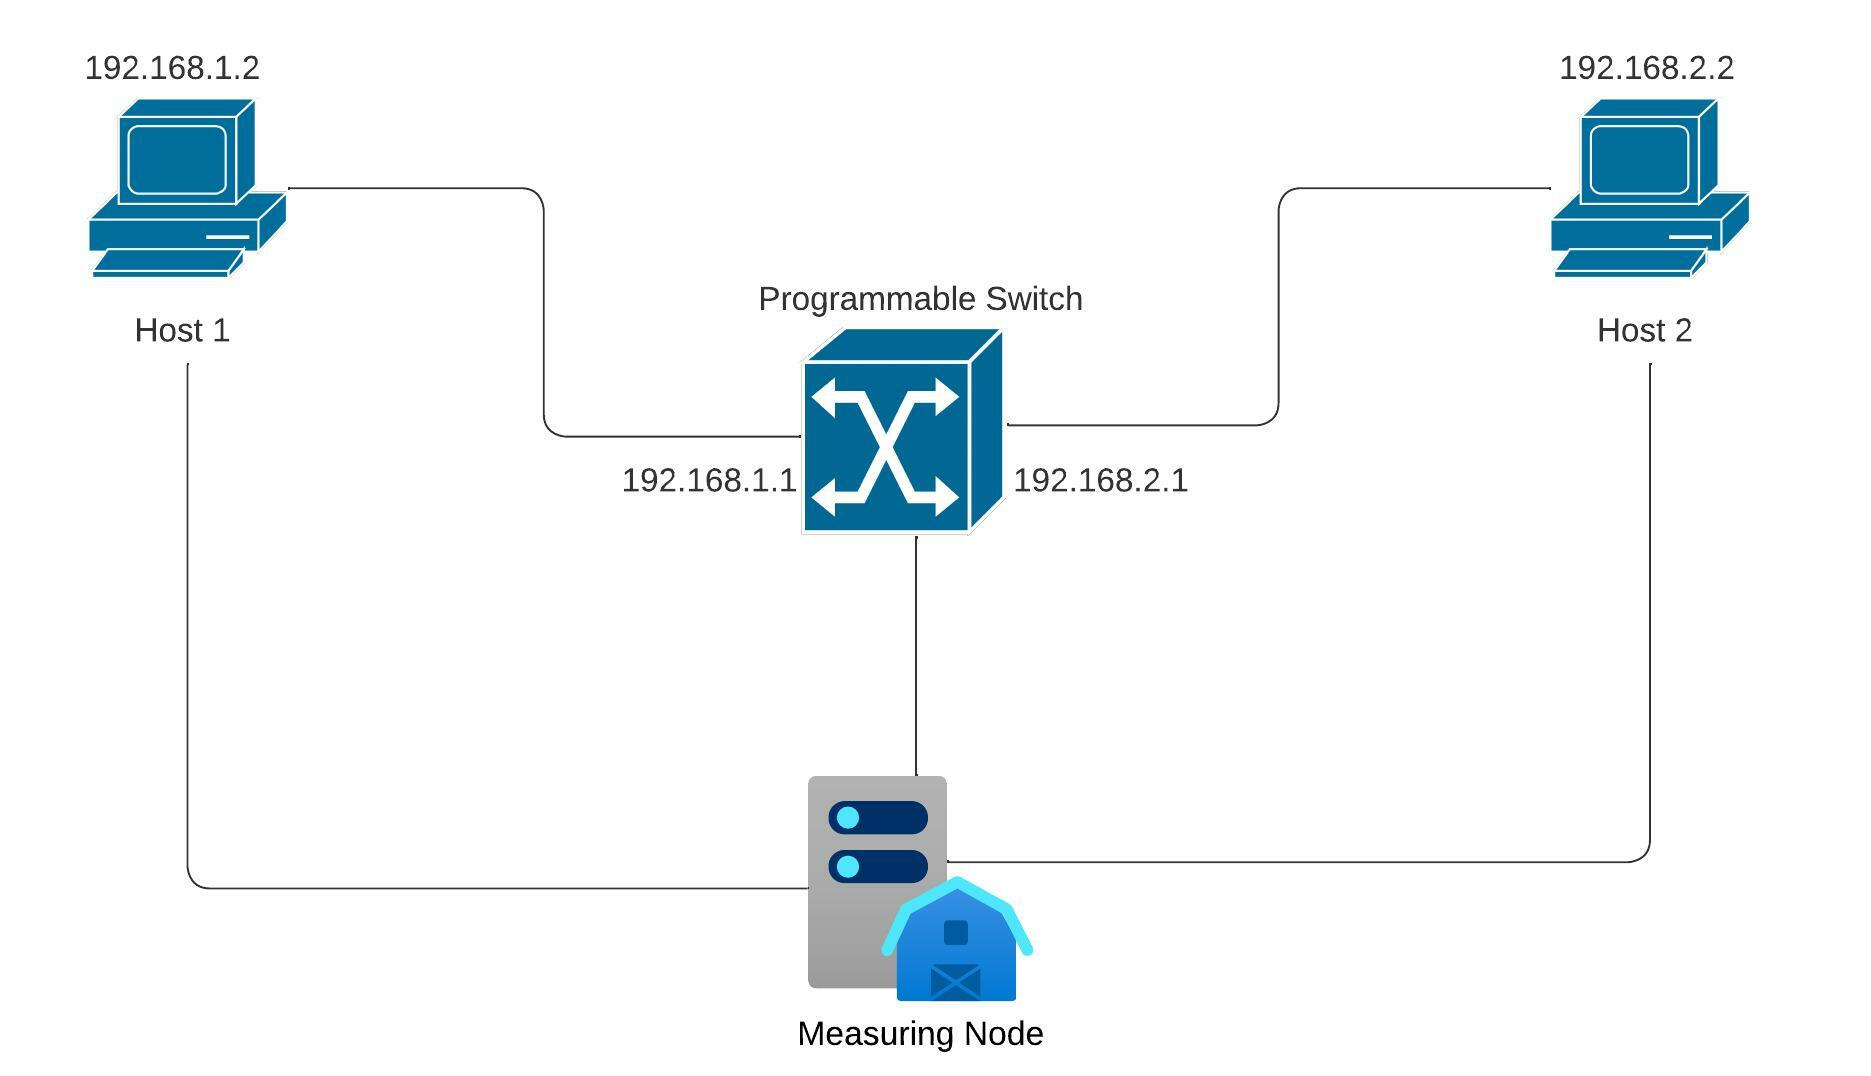
\includegraphics[scale=0.355]{Initial_Switch_Topology.jpeg}
        \centering
        \caption{Initial Experiment Topology}
    \end{figure}
    The motivation of this experiment is to gain a foundation in deploying programmable P4 switches on the FABRIC testbed, along with instantiating a measurement node using the MFLib API to collect the number of packets transmitted on the interfaces of each device. 
    \subsection{Final Experiment Setup}
    We describe the topology used for our final experiment in Figure 2. Here, two distinct paths between Hosts 1 and 2 are connected by programmable P4 switches. The measuring node of our infrastructure provided by the MFLib API will act as the controller to configure the optimal routing path to minimize the latency between the two hosts. The routing tables on the programmable switch will be configured dynamically to alternate between the two available paths between the hosts using the P4Runtime specification. 
    
    The measuring node is chosen to be the controller as it is connected to each device in the topology and has direct access to the overall slice-level metrics of the topology. This project's scope is to have only two routes between the hosts; however, in a real-world scenario, more than two routes can exist.
    
    To demonstrate the efficacy of our proposed algorithm, the experiment will be tested on cases in which one or more links of the routes connecting the two hosts have lower available bandwidth.
    \begin{figure}[h!]
        \centering
        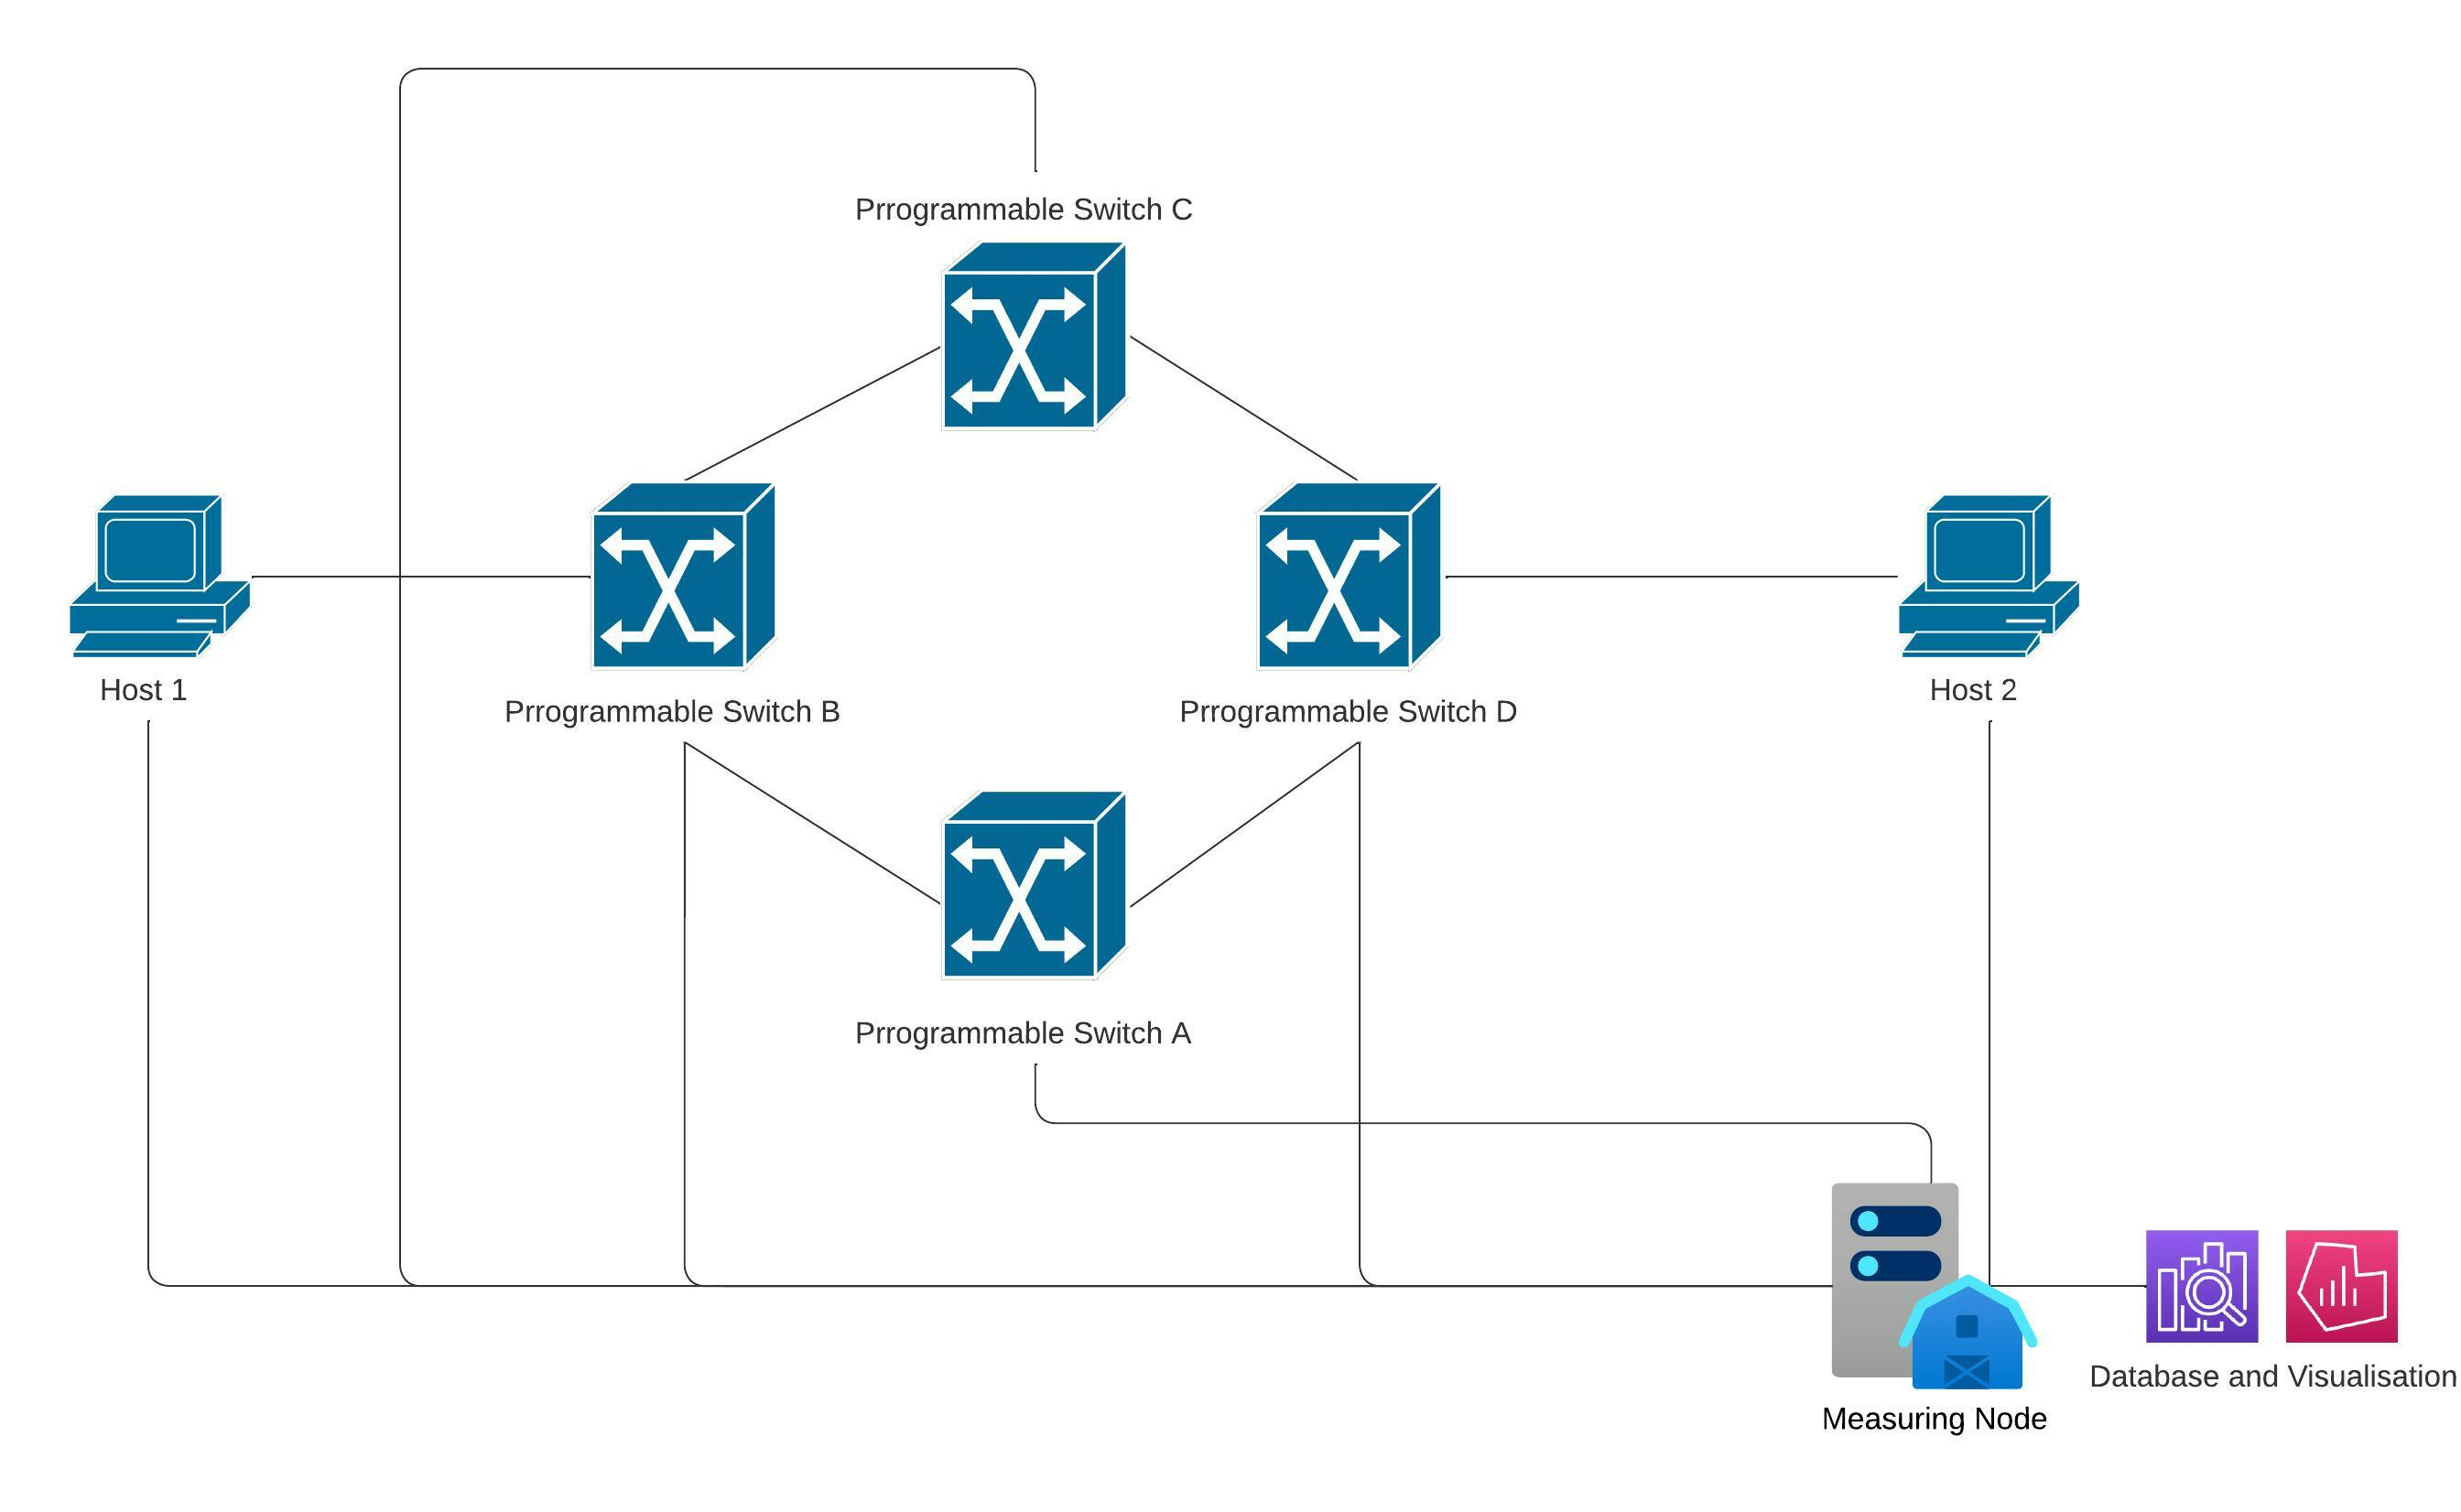
\includegraphics[scale=0.4]{Final_Switch_Topology.jpeg}
        \caption{Final Experiment Topology}
    \end{figure}
     
    \section{Methodology}
    \subsection{P4 Switch Deployment on FABRIC}
    	
     We create nodes with multiple basic network interface cards (NIC) for replicating switches on the FABRIC testbed.  
    \begin{figure}[h!]
            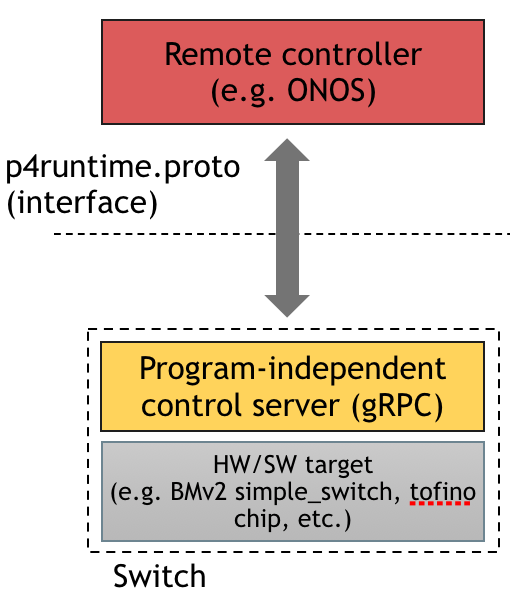
\includegraphics[scale=0.21]{P4Runtime.png}
            \centering
            \caption{Basic Working of P4Runtime}
    \end{figure}
    Each node is installed with the P4 compiler (P4C) specification, the Behavioral Model (BmV2), and their corresponding dependencies. BmV2 is the software switch target primarily used for testing and debugging programmable data planes. We deploy a basic packet forwarding P4 program on all our switches for our experiments. The packet forwarding tables are dynamically configured from the measurement node using the P4Runtime specification. P4Runtime executes switch-level configurations using remote procedure calls (RPCs) and protocol buffers (ProtoBuf) (as illustrated in Figure 3) and also has wrapper functions written for Python and Go.
     

        \subsection{Metrics Collection using the MFLib API}
    The complete slice-level metrics will be measured using the MFLib API present on the FABRIC testbed. It enables us to have a definitive way to store our metrics using Prometheus, the logs using ElasticSearch (ELK stack), and visualize the collected data using Kibana and Grafana. There are two steps for adding the measurement framework to a slice topology: 
    
    \subsubsection{Measurement Node Creation}: The first step is to create a new measurement node that connects to each node present in the original topology through a single network connection. This is illustrated in Figure 4. A critical limitation of this step is the requirement that each node must belong on the same testbed site.
    
    \begin{figure}[h]
        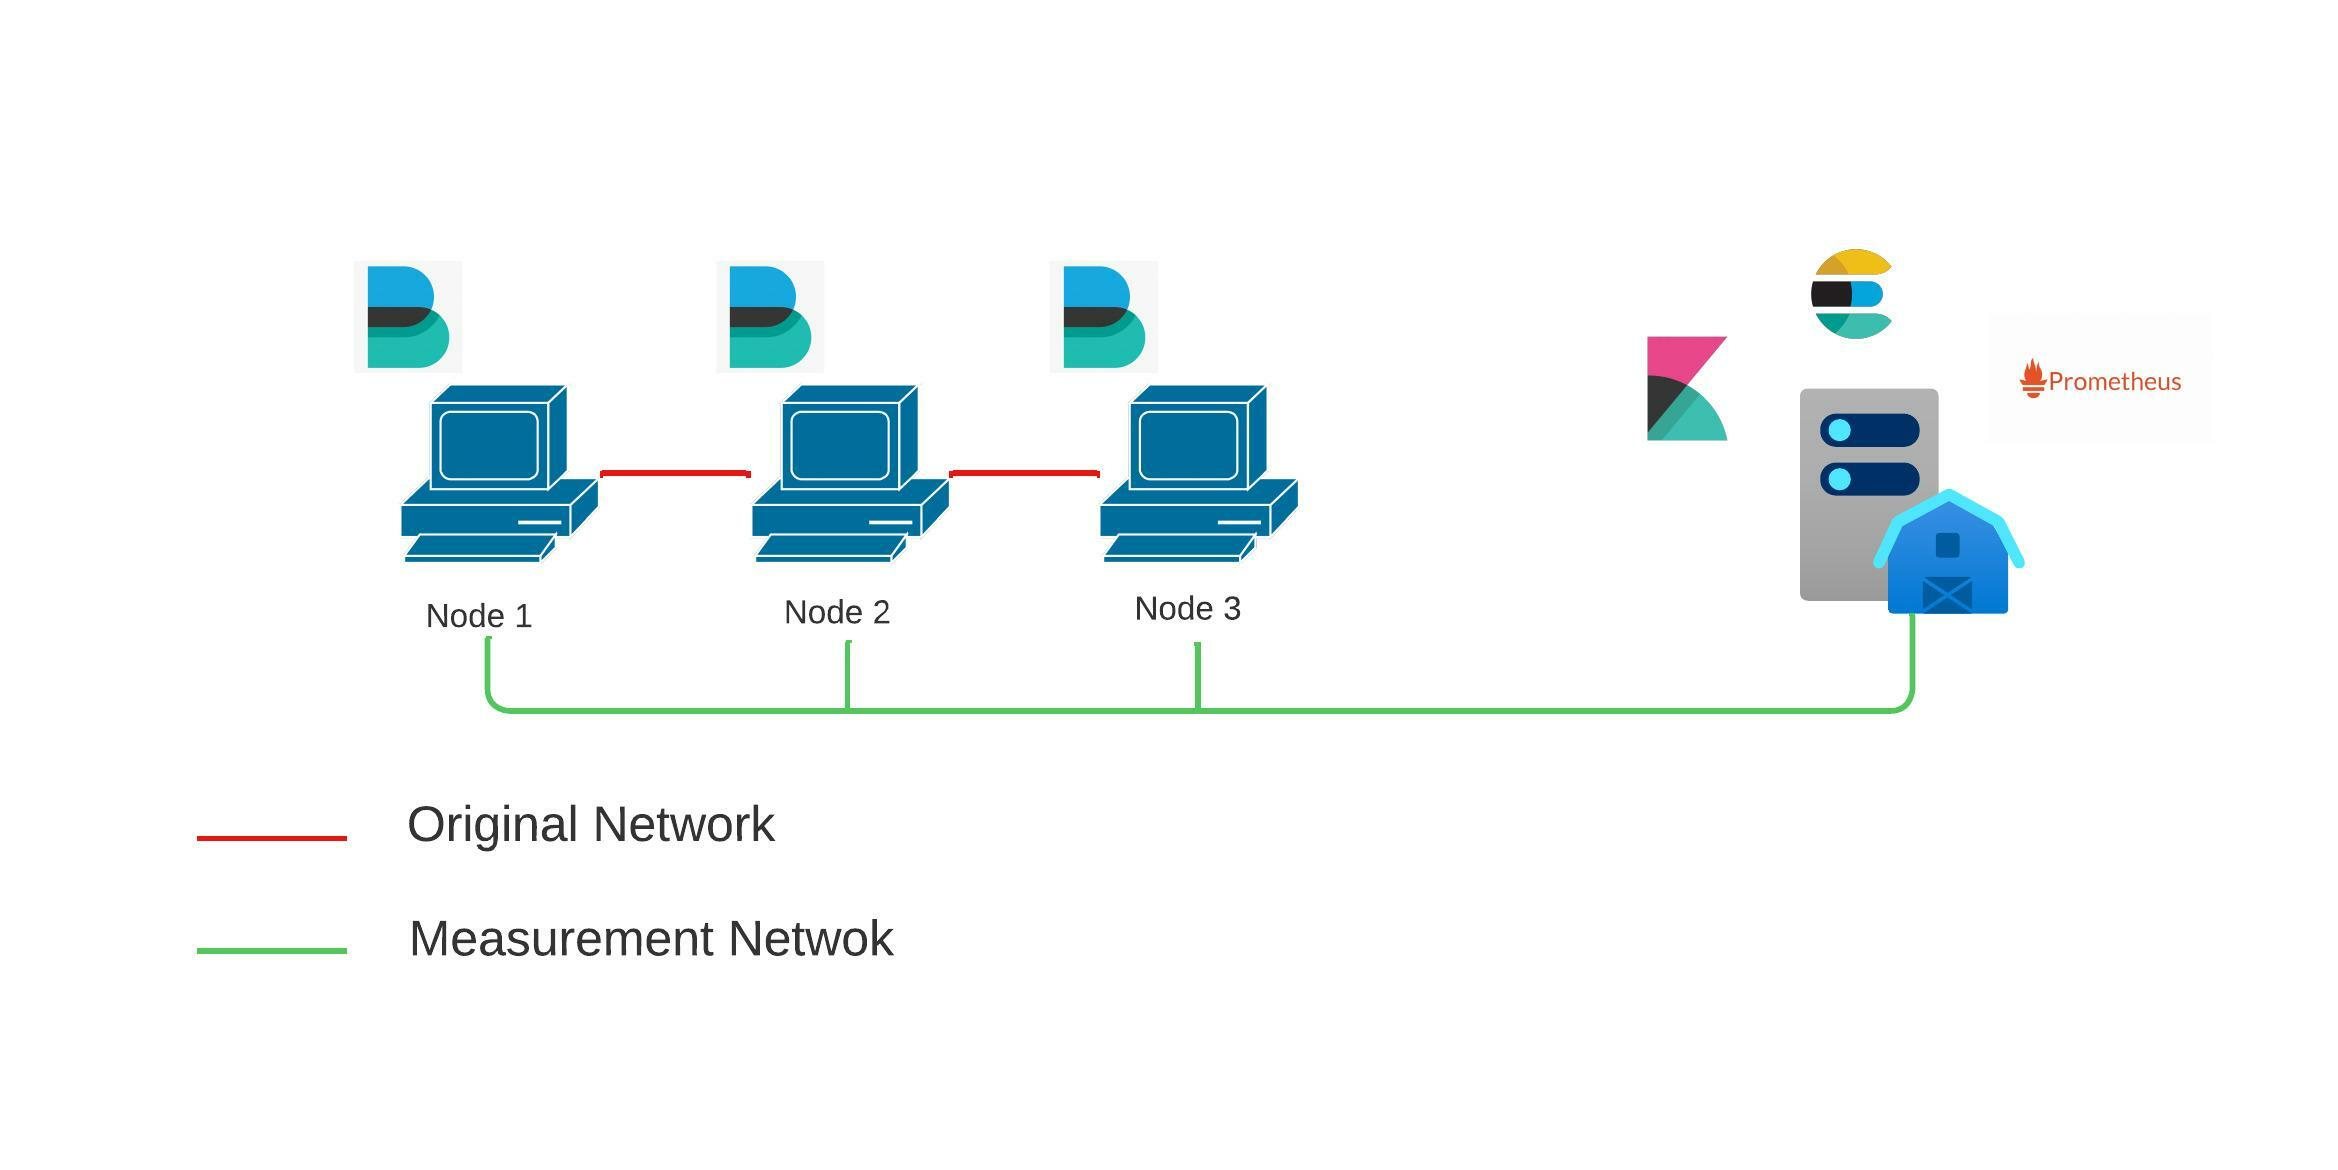
\includegraphics[scale=0.45]{Mflib.jpeg}
        \centering
        \caption{Architecture consisting of the Measurement Framework on a Network Slice}
    \end{figure}
    
    \subsubsection{Initating the overall Slice Instrument} The second step is to configure Prometheus for the collection parameters from each interface present in the topology and upload the required dashboards to the Kibana and Grafana servers.

    
    The measuring node collects and stores the device-level metrics, such as TCP/ICMP/UDP packets (in/out) and queue buffering length for each network interface, and overall slice-level metrics, such as system load and network traffic load. We write customized python wrapper functions to access these metrics used in our core algorithm.

    \subsection{Network Traffic Generation}
    We use scapy as our traffic generator to modulate the load on the different routes between our hosts. Scapy is a python program that enables users to send, sniff, dissect, and forge network packets. Scapy is prominently used to construct tools that can probe, scan or attack networks.

    \subsection{Dynamic Routing Algorithm}
      Before packet transmission from one host to another, the controller (in our experiment, the measurement node) will evaluate the optimal packet forwarding route based on the minimum cumulative sum of two separate device-level metrics:
      \begin{enumerate}
          \item Available bandwidth of each link on the route. 
          \item Transmit + Receiving buffer lengths of each interface on the route.
      \end{enumerate}
      This algorithm will also be adapted for cases of link failure, and the resulting optimal packet forwarding route will be configured according to what was discussed in section V.

    \section{Results}
    \subsection{Initial Experiment Results}
    Our initial experiment demonstrates the implementation of a network slice consisting of a single programmable switch topology monitored by the measurement node based on the MFLib API. A basic packet forwarding P4 program is loaded and compiled on the programmable switch.
    \begin{figure}[b]
        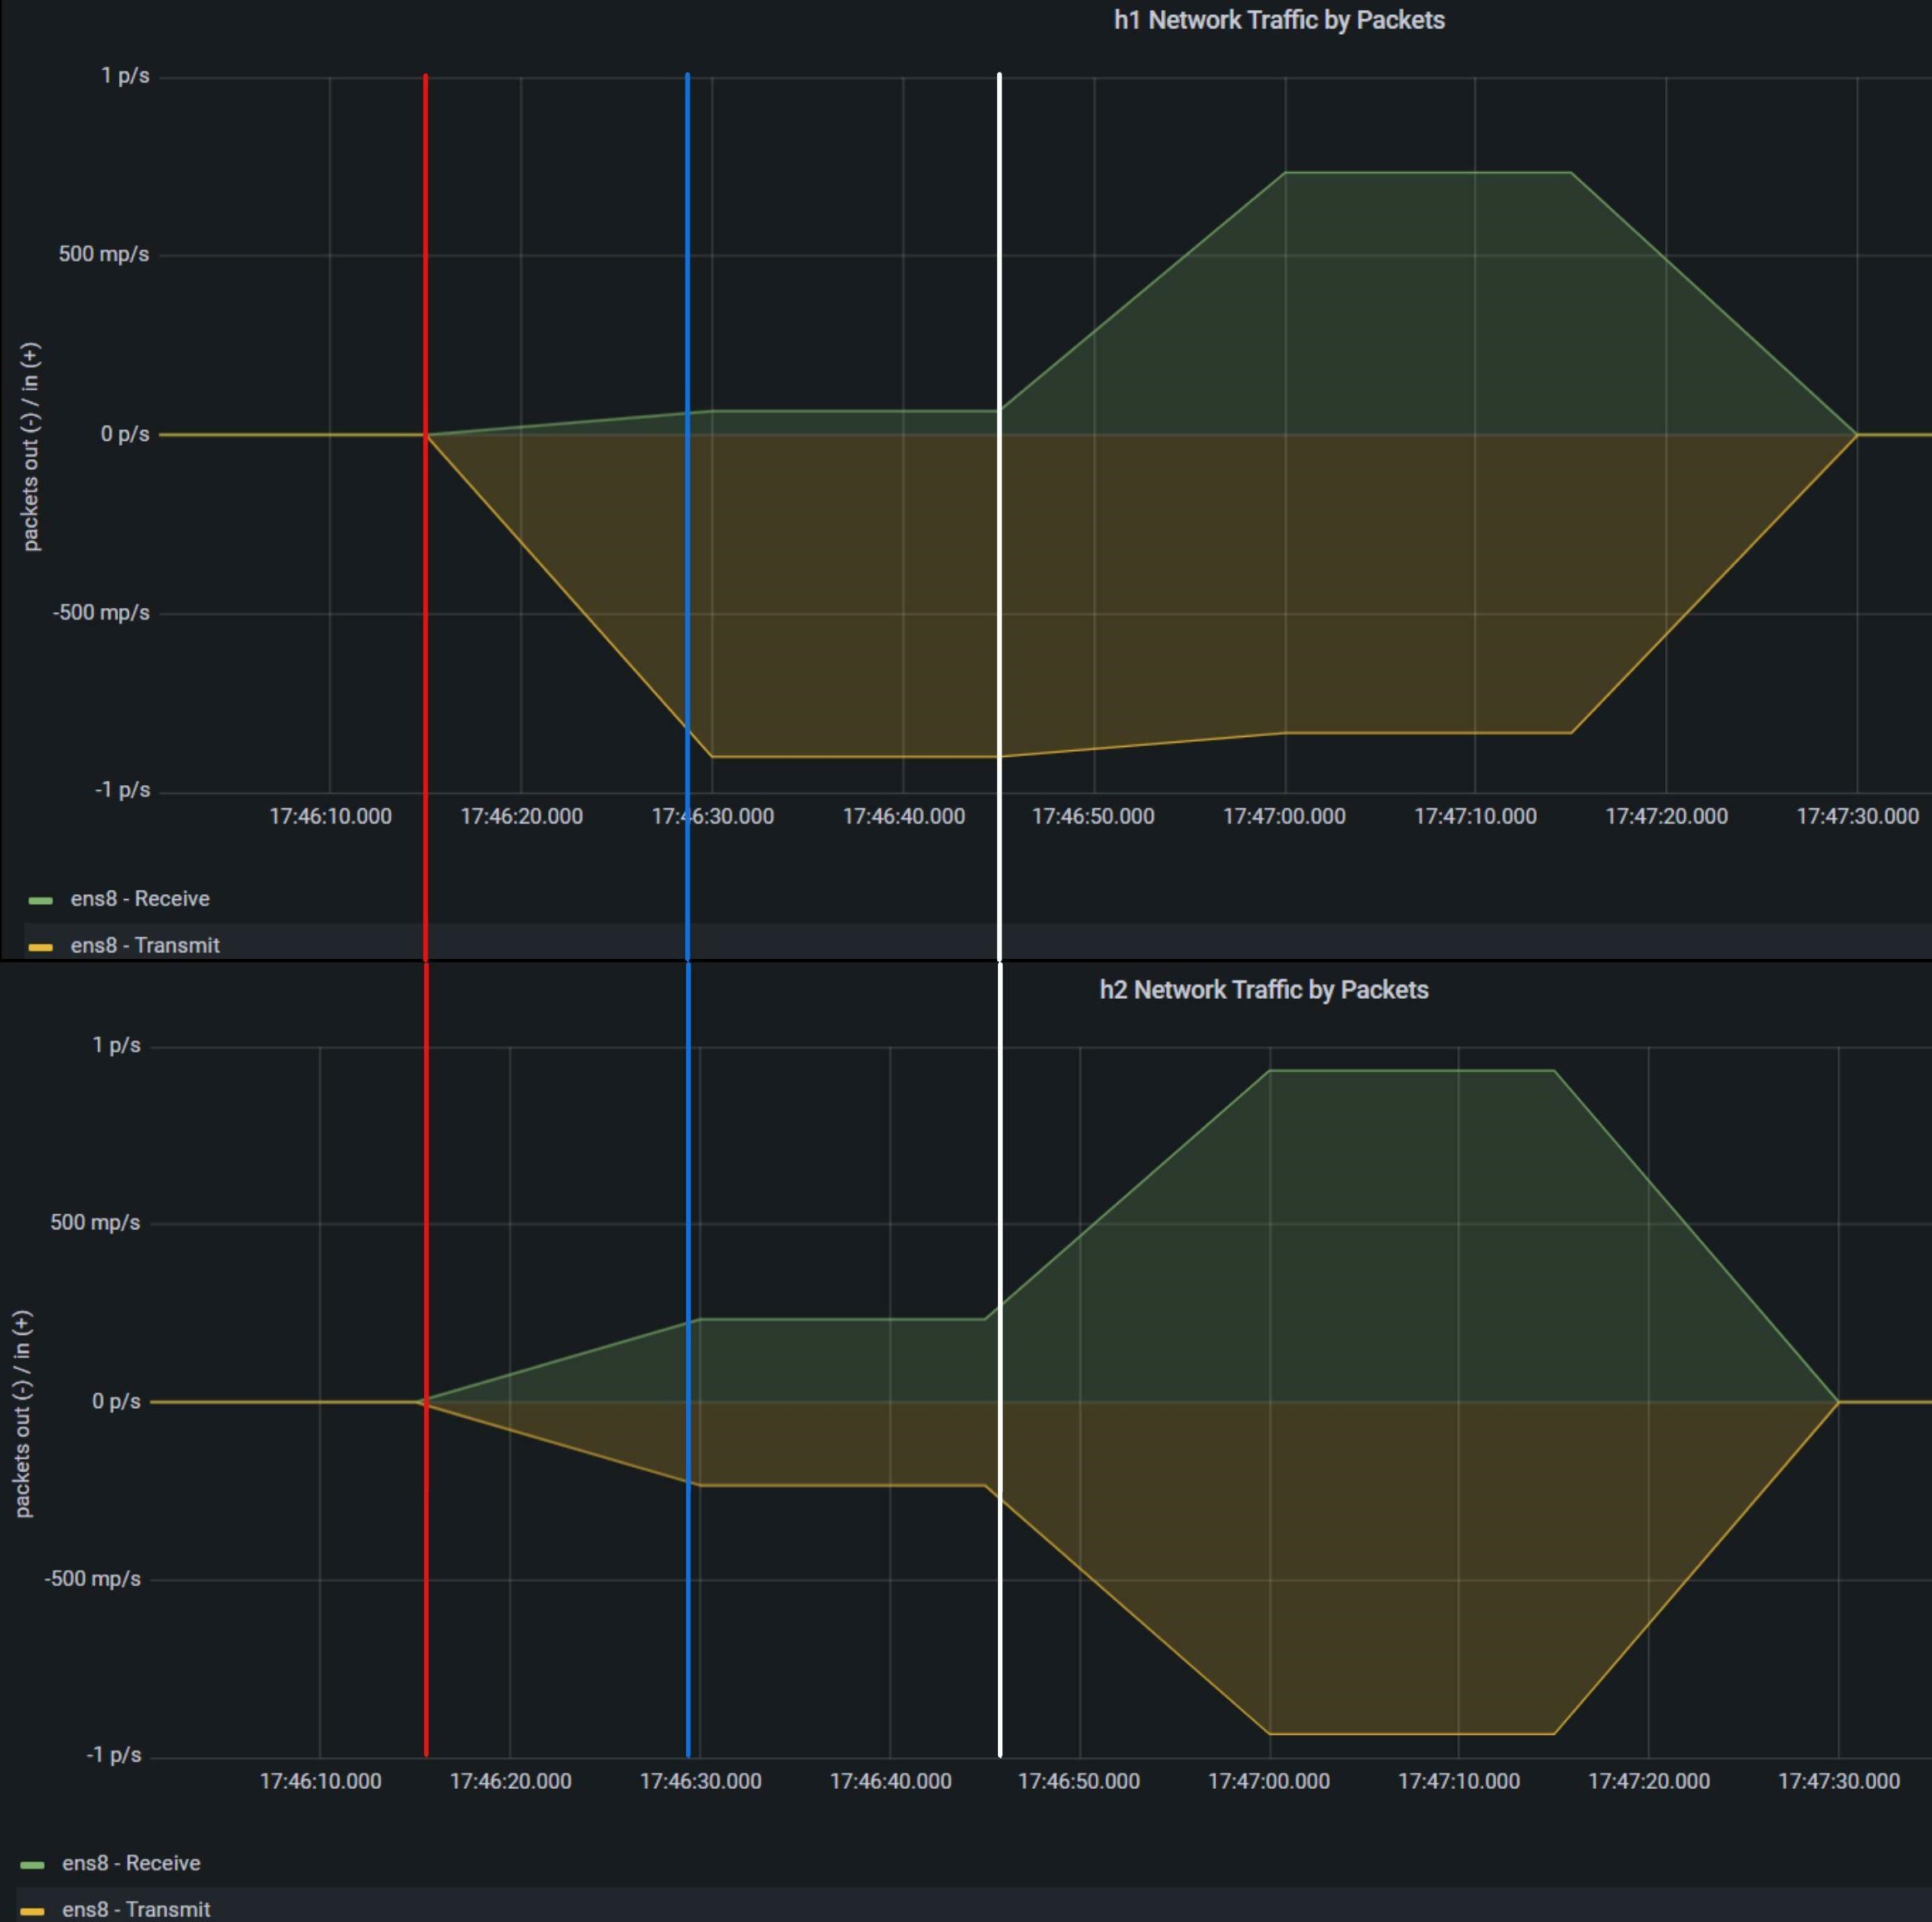
\includegraphics[scale=0.4]{packetgraph.jpeg}
        \centering
        \caption{Initial Results: Ping Statistics from Host 1 (top) to Host 2 (bottom)}
    \end{figure}
    
    In Figure 5, we showcase the ping statistics (ICMP packets) from Host 1 to Host 2, measured using the MFLib API and visualized using Grafana.
    Initially, the switch is not configured with any packet forwarding routes. At point 1 (marked by the red vertical line in Figure 5), Host 1 begins transmitting packets to the switch with Host 2 as the destination. As no routes are configured on the switch, Host 2 receives no traffic, and Host 1 does not receive any responses.

    At point 2 (marked by the blue vertical line in Figure 5), we configure the forward route from the switch to Host 2. At this point, Host 2 starts receiving the ICMP packets from Host 1 and sends back responses addressing Host 1. Note that the reverse route (from switch to Host 2) is yet to be configured.

    At point 3 (marked by the white vertical line in Figure 5), we configure the reverse route from the switch back to Host 1. At this point, Host 1 starts receiving the ICMP responses from Host 2. In Figure 6, we provide a snapshot of the routing tables on the programmable switch after configuring the forward and reverse routing paths.

    \begin{figure}[t]
        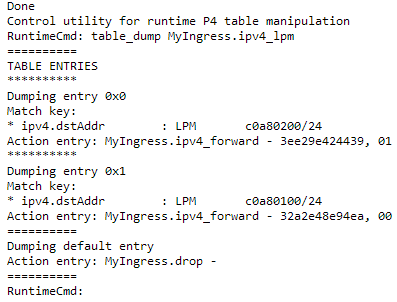
\includegraphics[scale=0.5]{Switch_Routing_Table.png}
        \centering
        \caption{Initial Results: P4 Routing Table on Switch}
    \end{figure}
        
    \subsection{Final Experiment Results}
    ---- to be added ----

    \section{Conclusions and Summary}
    ---- to be added ----
    
    \section{Learning Outcomes and Future Work}
    The primary learning of this project is to gain a deep understanding of P4, its implementation details, and how to deploy and configure programmable switch networks efficiently. We also hope that our work on the FABRIC measurement framework can be used as a platform for creating more complex network measurement framework-based experiments on FABRIC in the future.
        
    Potential future work based on this project can include the analysis of the INT framework using a P4 switch topology. This extension can consist of role enhancements to each switch in the topology to create an efficient monitoring and telemetry system with minimal latency overheads. A comparison of the metrics collected using MFLib and the INT framework can be visualized using Grafana and Kibana. The primary challenge in setting up the INT-based telemetry system is to minimize network and processing overheads of the INT packets while still collecting sufficient metrics to represent the flow state of the network accurately.

    \section{Acknowledgements}
    First and foremost, we would like to extend our gratitude to our professor, Dr. Violet Syrotiuk, who has played an instrumental role at all stages of this project. We want to thank her for allowing us to work on the FABRIC testbed, our first foray into using experimental testbeds, and for providing us with resources and tutorials on the P4 programming language. We also want to thank Dr. Jorge Crichigno of the University of South Carolina for providing us access to his high-quality tutorials on the P4 programming language.

    \begin{thebibliography}{00}
        \bibitem{b1} Pat Bosshart, Dan Daly, Glen Gibb, Martin Izzard, Nick McKeown, Jennifer Rexford, Cole Schlesinger, Dan Talayco, Amin Vahdat, George Varghese, and David Walker. 2014. "P4: programming protocol-independent packet processors". SIGCOMM Comput. Commun. Rev. 44, 3 (July 2014), 87–95

        \bibitem{b2} Weverton Luis da Costa Cordeiro, Jonatas Adilson Marques, Luciano Paschoal Gaspary, "Data Plane Programmability Beyond OpenFlow: Opportunities and Challenges for Network and, Service Operations and Management." Journal of Network and Systems Management (September 2017).

        \bibitem{b3} Ilya Baldin, Anita Nikolich, Paul Ruth, Jim Griffioen, Kuang-Ching Wang, Inder Monga, and Tom Lehman, "FABRIC Functional Design," v0.4

        \bibitem{b4} Ilya Baldin, Anita Nikolich, Paul Ruth, Jim Griffioen, Kuang-Ching Wang, Inder Monga, and Tom Lehman, "FABRIC Measurement Framework Design," v0.2

        \bibitem{b5} Maria Apostolaki, Ankit Singla, and Laurent Vanbever. 2021. Performance-Driven Internet Path Selection. In Proceedings of the ACM SIGCOMM Symposium on SDN Research (SOSR) (SOSR '21). Association for Computing Machinery, New York, NY, USA, 41–53. https://doi.org/10.1145/3482898.3483366

        \bibitem{b6} The P4.org Applicattwoons Working Group. Contributions from Alibaba, Arista, CableLabs, Cisco Systems, Dell, Intel, Marvell, Netronome, VMware, "In-band Network Telemetry (INT) Dataplane Specification," Version 2.1, 2020-11-11

        \bibitem{b7} N. Van Tu, J. Hyun, and J. W.-K. Hong, "Towards ONOS-based SDN monitoring using in-band network telemetry," in Proc. 19th Asia–Pacific Netw. Oper. Manage. Symp. (APNOMS), Seoul, South Korea, Sep. 2017, pp. 76–81

        \bibitem{b8} N. V. Tu, J. Hyun, G. Y. Kim, J. -H. Yoo and J. W. -K. Hong, "INTCollector: A High-performance Collector for In-band Network Telemetry," 2018 14th Interconsist of Conference on Network and Service Management (CNSM), 2018, pp. 10–18.

        \bibitem{b9} Xiaoqi Chen, Hyojoon Kim, Javed M. Aman, Willie Chang, Mack Lee, and Jennifer Rexford. 2020. Measuring TCP Round-Trip Time in the Data Plane. In Proceedings of the Workshop on Secure Programmable Network Infrastructure (SPIN '20). Association for Computing Machinery, New York, NY, USA, 35–41. https://doi.org/10.1145/3405669.3405823
    \end{thebibliography}
    

\end{document}
